% Chapter Template

\chapter{Bug Fixing} % Main chapter title

\label{Chapter 7} % Change X to a consecutive number; for referencing this chapter elsewhere, use \ref{ChapterX}

This chapter will describe issues found during the project, but were not covered in the previous chapters. In addition to describing the issues, if applicable, the corrections to resolve these issues will be given. If the issues were unresolved, a suggestion at the possible causes for the issue will be given. Section \ref{Ch7 Sec1} details the issues discovered during matrix mode.

%----------------------------------------------------------------------------------------
%	SECTION 1
%----------------------------------------------------------------------------------------

\section{Matrix Mode Bugs}

\label{Ch7 Sec1}

As discussed in chapter \ref{Chapter 5}, by implementing letterboxing into matrix mode several minor bugs were also introduced.

%-----------------------------------
%	SUBSECTION 1
%-----------------------------------

\subsection{Character Duplication}

\label{Ch7 Sec1 Sub1}

After letterbox implementation, a strange phenomenon occurred on the left side of the screen when in matrix mode. It appears that there is a region, about four character wide, that contains duplicates of characters from the next line. In addition to this duplicate, there appears to be smearing of the first two characters in this duplicate region. These observations can be seen in figure \ref{fig:matrixmodecharacterinputerror}. In addition to the issues with the left region, it is believed that these issues are causing the screen to become shifted to the right. As seen in figure \ref{fig:matrixmodecharacterinputerror}, the characters are continuing past the right most visible point of the screen. 

\begin{figure}
  \centering
  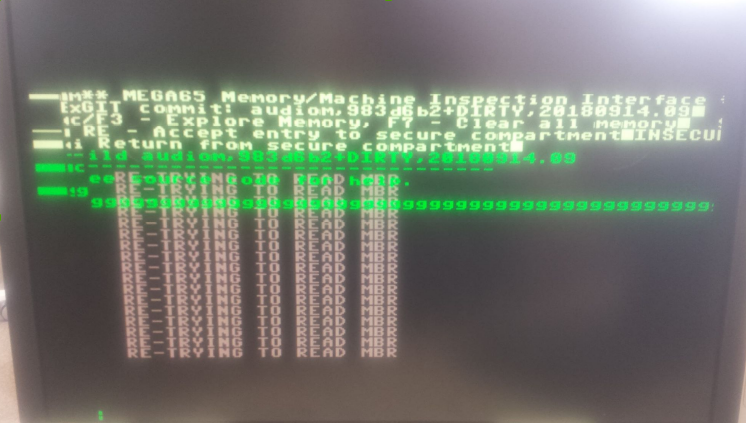
\includegraphics[width=\linewidth]{matrixmodecharacterinputerror}
  \caption{The matrix rain compositor smearing / duplication.}
  \label{fig:matrixmodecharacterinputerror}
\end{figure}

%----------------------------------------------------------------------------------------
%	SECTION 2
%----------------------------------------------------------------------------------------

\section{Secure Compartmentalisation Bugs}

\label{Ch7 Sec2}

\subsection{SD Card Issue}

\label{Ch7 Sec2 Sub1}

When implementing the secure compartmentalisation, it was noted that there was an anomoly when attemping to write to the SD card. When attempting to write to the SD card, the write actions would perform as expected, but no data would be written; instead the sector that was to be written to was erased. As no dedicated erase function had be developed, this was expected to be the FPGA attempting to write to the SD card, not meeting the power requirements to successfuly write. This would cause the data seen from the SD card to be all logic low and the write proccess to complete successfuly, thus throwing no errors. Changing the FPGA power supply from USB to the mains outlet fixed these issues.

